%%%%%%%%%%%%%%%%%%%%%%%%%%%%%%%%%%%%%%%%%%%%%%%%%%%%%%%%%%%%%%%%%%%%%%%%
% Plantilla TFG/TFM
% Universidad de Murcia. Facultad de Informática
% Realizado por: José Manuel Requena Plens
% Modificado: Pablo José Rocamora Zamora
% Contacto: pablojoserocamora@gmail.com
%%%%%%%%%%%%%%%%%%%%%%%%%%%%%%%%%%%%%%%%%%%%%%%%%%%%%%%%%%%%%%%%%%%%%%%%


\chapter{Introducción}

El entrenamiento de redes neuronales profundas para el análisis de tomogramas de crio-microscopía
electrónica (\textit{cryo-ET}) exige grandes volúmenes de datos anotados cuya obtención
experimental es inviable a escala. La generación de tomogramas sintéticos —volúmenes simulados
con distribuciones realistas de proteínas, membranas y ruido— es la alternativa más extendida
para producir conjuntos de entrenamiento a bajo coste. La calidad de esos datos sintéticos
depende directamente de cuán eficientemente el software de simulación consigue empaquetar
macromoléculas en el volumen de interés.\\

\textit{PolNet}~\cite{martinezSanchezPolnetGithub}, el marco de simulación de referencia en este ámbito, emplea el algoritmo
\textit{SAWLC} (\textit{Self-Avoiding Worm-Like Chain}) para insertar proteínas en el
volumen. SAWLC produce distribuciones biológicamente plausibles, pero su carácter secuencial y
sus altas tasas de rechazo en volúmenes densos hacen que la generación de un único tomograma
pueda requerir entre 30 y 45 minutos sin alcanzar el grado de empaquetamiento deseado, 
lo que limita severamente la escala de producción de datos.\\

\begin{figure}[h]
     \centering
     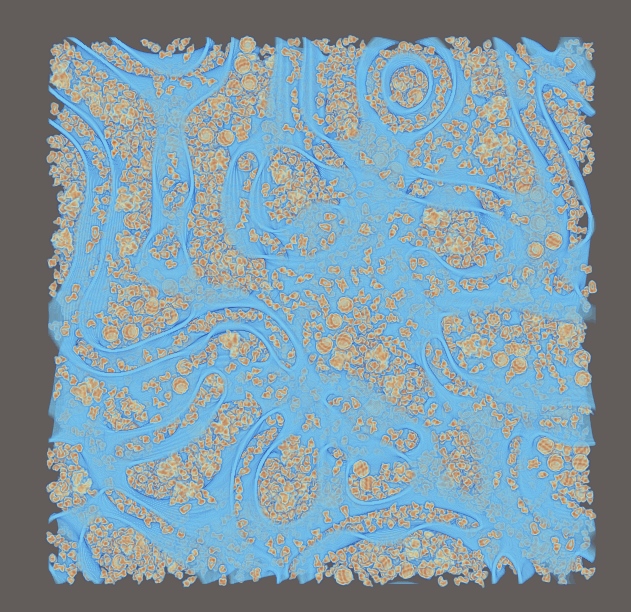
\includegraphics[width=0.5\textwidth]{archivos/sawlc-tomo.png}
     \caption{Tomograma generado con la inserción SAWCL.}
     \label{fig:sawcl-tomo}
\end{figure}

Este Trabajo Fin de Grado adapta e implementa \textbf{Tetris}~\cite{harastani2025template_repo}, un algoritmo de inserción de
proteínas basado en correlación cruzada 3D mediante FFT que, en cada paso, identifica
globalmente la posición óptima de colocación en lugar de muestrear candidatos al azar. El
algoritmo se adapta para operar en volúmenes que ya contienen estructuras biológicas
preexistentes (como membranas generadas por PolNet) y se extiende con un
mecanismo de crecimiento por clústeres guiado por semilla. Se desarrolla además una versión
acelerada por GPU con \textit{CuPy} que dirige automáticamente las operaciones más costosas
(correlación FFT 3D y muestreo global de semilla mediante \texttt{argwhere}) a la tarjeta
gráfica, manteniendo la misma lógica algorítmica que la versión
CPU. El trabajo se articula en un {repositorio independiente}~\cite{Hamo2025tetris_rep} cuyo objetivo es comparar Tetris
frente a SAWLC y evaluar si constituye un reemplazo viable para el módulo de inserción de
PolNet.\\

\begin{figure}[h]
     \centering
     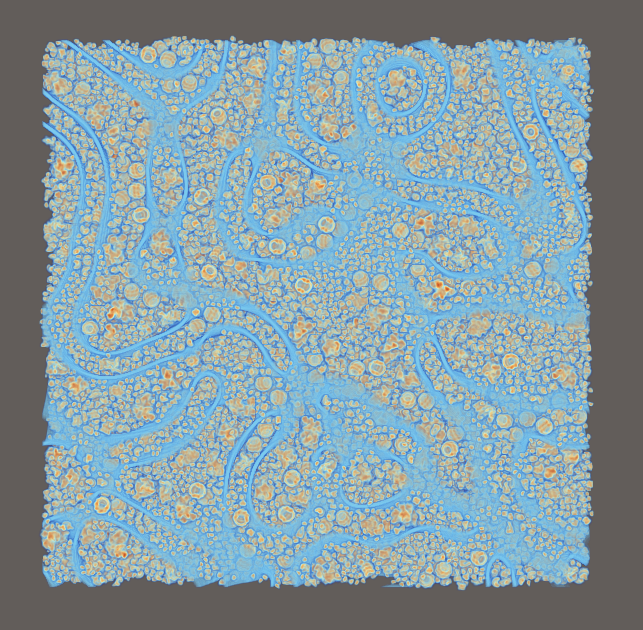
\includegraphics[width=0.5\textwidth]{archivos/tomo-tetris.png}
     \caption{Tomograma generado con la inserción Tetris.}
     \label{fig:sawcl-tomo}
\end{figure}

Los objetivos concretos del trabajo son: (i)~adaptar el algoritmo Tetris con correlación FFT
3D al contexto de PolNet, incorporando la información de membranas preexistentes y un
mecanismo de crecimiento por clústeres guiado por semilla; (ii)~desarrollar una versión
acelerada por GPU sobre \textit{CuPy} y rutas duales
CPU/GPU transparentes; (iii)~diseñar un banco de pruebas que compare ambos algoritmos en
ocupancia volumétrica, número de monómeros insertados y tiempo de ejecución; y
(iv)~analizar en qué escenarios Tetris supone una alternativa competitiva a SAWLC.\\

El resto del documento se organiza como sigue. El Capítulo~2 revisa el estado del arte:
fundamentos de la adquisición cryo-ET, métodos de generación de datos sintéticos y el
funcionamiento de SAWLC en el contexto de PolNet. El Capítulo~3 recoge el análisis de
requisitos. El Capítulo~4 describe el diseño e implementación de Tetris y del banco de
pruebas. El Capítulo~5 presenta y discute los resultados experimentales. El Capítulo~6 cierra
con las conclusiones y las líneas de trabajo futuro.
